\documentclass[aspectratio=169]{beamer}
\usepackage[utf8]{inputenc}
\usepackage{tikz} % for QR code overlay

% code snippets
\usepackage{minted}
\newmintedfile[dockercode]{dockerfile}{
  % bgcolor=mintedbackground,
  fontfamily=tt,
  linenos=true,
  numberblanklines=true,
  numbersep=5pt,
  gobble=0,
  frame=leftline,
  framerule=0.4pt,
  framesep=2mm,
  funcnamehighlighting=true,
  tabsize=4,
  obeytabs=false,
  mathescape=false
  samepage=false, %with this setting you can force the list to appear on the same page
  showspaces=false,
  showtabs =false,
  texcl=false,
}
\newminted[bashcode]{bash}{
  % bgcolor=mintedbackground,
  fontfamily=tt,
  linenos=true,
  numberblanklines=true,
  numbersep=5pt,
  gobble=0,
  frame=leftline,
  framerule=0.4pt,
  framesep=2mm,
  funcnamehighlighting=true,
  tabsize=4,
  obeytabs=false,
  mathescape=false
  samepage=false, %with this setting you can force the list to appear on the same page
  showspaces=false,
  showtabs =false,
  texcl=false,
}

% biblatex (requires biber; sudo pacman -S biber)
\usepackage[]{biblatex} % biblatex
\addbibresource{"./content/bib/bib1.bib"}
\addbibresource{"./content/bib/bib2.bib"}
\addbibresource{"./content/bib/throwaway.bib"}

\usepackage{graphicx}
\graphicspath{ {./content/img/} }

\usetheme{Boadilla}
\usecolortheme{rose}
% \beamerdefaultoverlayspecification{<+->} % this will turn it into slides

\title{Augmented Agronomist}
\subtitle{LAR Mini-Conference \today}
\author{George Onoufriou, Marc Hanheide, Georgios Leontidis}
\date{\today}

\begin{document}

\addtobeamertemplate{frametitle}{}{%
\begin{tikzpicture}[remember picture,overlay]
\node[anchor=north east,yshift=2pt] at (current page.north east) {
\includegraphics[height=1.5cm]{qrcode.png}};
\end{tikzpicture}}

  \frame{\titlepage}

  % \begin{frame}
  %   \frametitle{About}
  %   \begin{columns}
  %     \begin{column}{0.5\textwidth}
  %       \begin{itemize}
  %         \item PhD Candidate Computer/ Data Science
  %         \item Privacy and Linux Enthusiast
  %       \end{itemize}
  %     \end{column}
  %     \begin{column}{0.5\textwidth}
  %       \begin{figure}[th!]
  %         \centering
  %         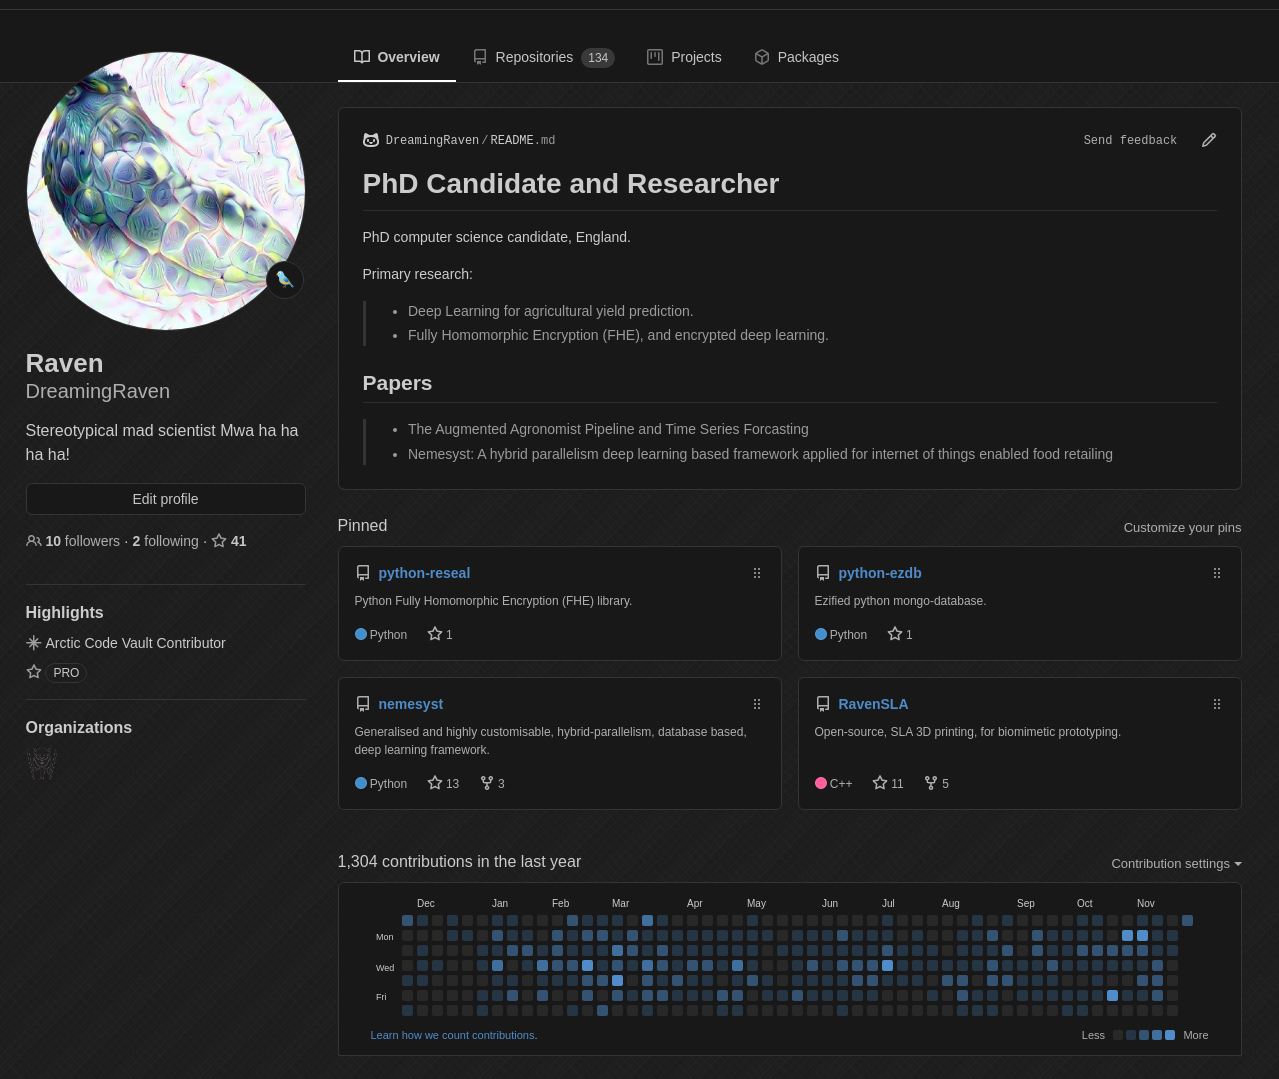
\includegraphics[width=0.8\textwidth]{gh.png}
  %         \caption{GitHub profile page where you can come to see my work and chat. \autocite{repository}}
  %         \label{fig:gh}
  %       \end{figure}
  %     \end{column}
  %   \end{columns}
  % \end{frame}

  \begin{frame}
    \frametitle{Augmented Agronomist}
    \begin{columns}
      \begin{column}{0.5\textwidth}
        The Augmented Agronomist is:
        \begin{itemize}
          \item Privacy-Preserving Deep Learning
          \item (Un)Certainty Metrics
          \item Robotic Attention
        \end{itemize}
        Applied to:
        \begin{itemize}
          \item Agriculture; Predicting plant yield, in particular strawberries.
          \item How certain we are of our predictions.
          \item Given uncertain or problematic scenarios get robot to re-investigate.
        \end{itemize}
      \end{column}
      \begin{column}{0.5\textwidth}
        \begin{figure}[th!]
          \centering
          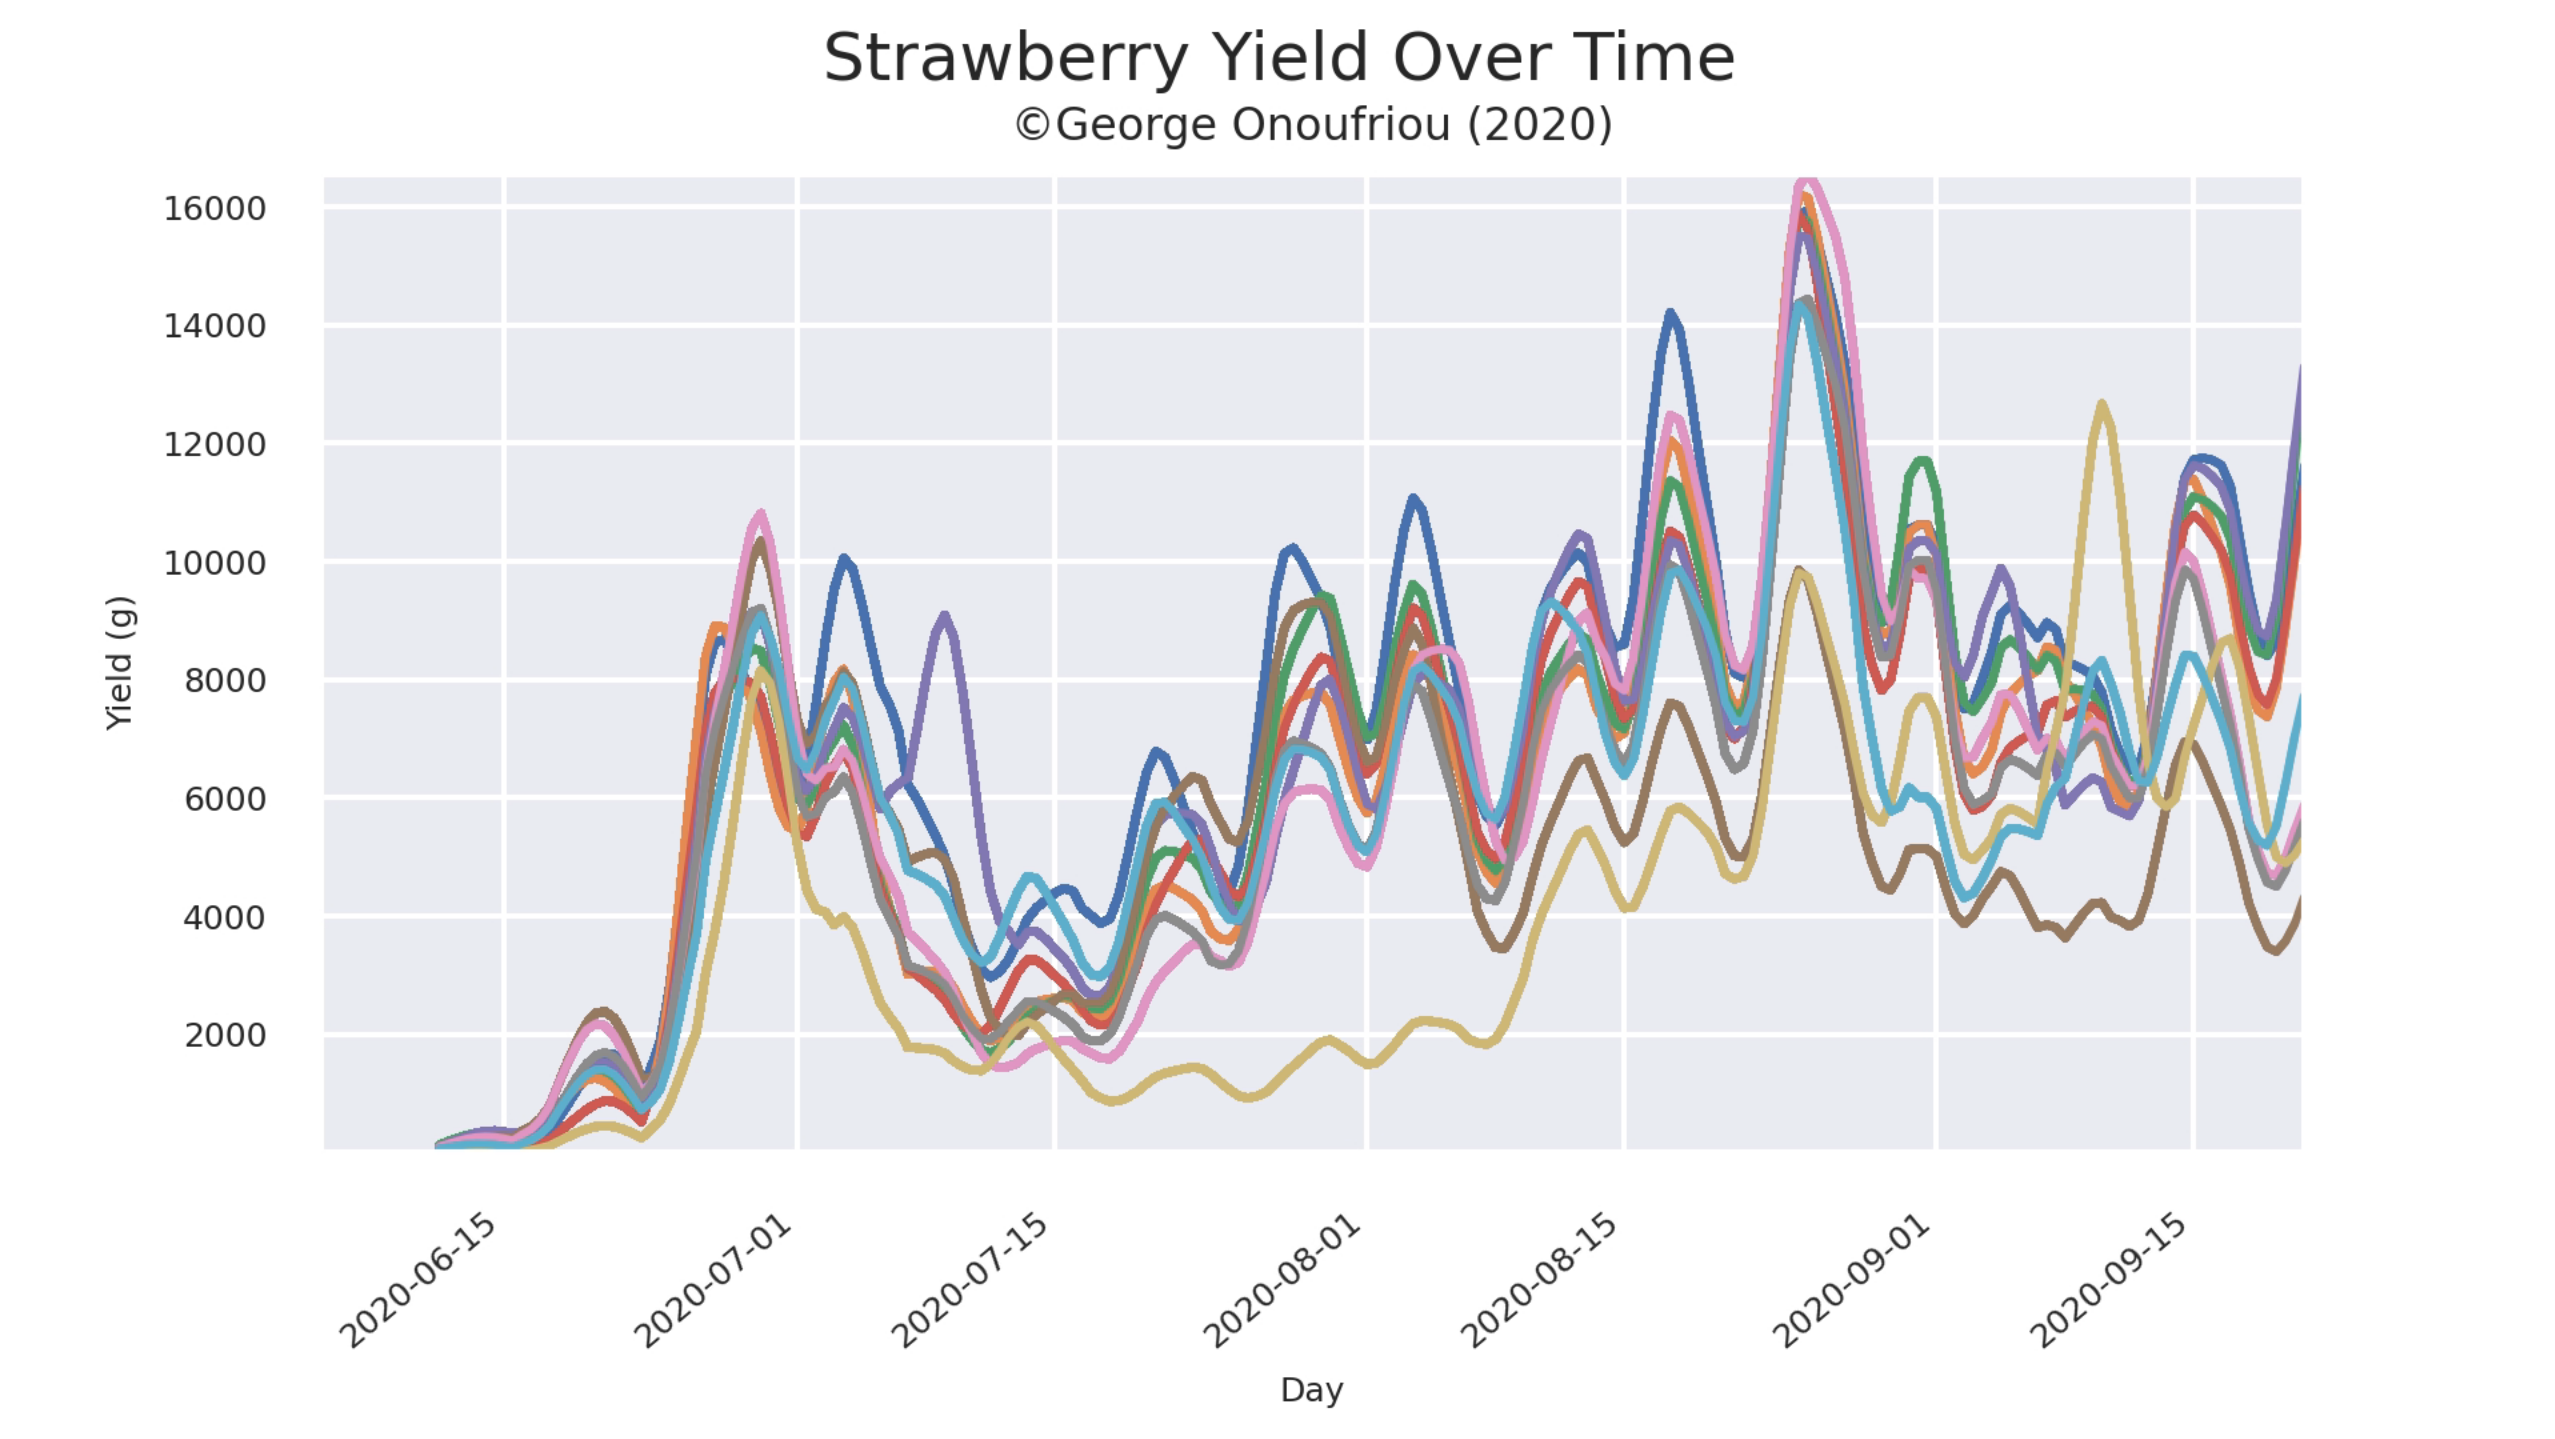
\includegraphics[origin=c,width=1\textwidth]{yield.png}
          \caption{Yield over time in our riseholme campus (2020).}
          \label{fig:yield}
        \end{figure}
      \end{column}
    \end{columns}
  \end{frame}

  \begin{frame}
    \frametitle{Augmented Agronomist Predictions}
    \begin{columns}
      \begin{column}{0.5\textwidth}
        \begin{figure}[th!]
          \centering
          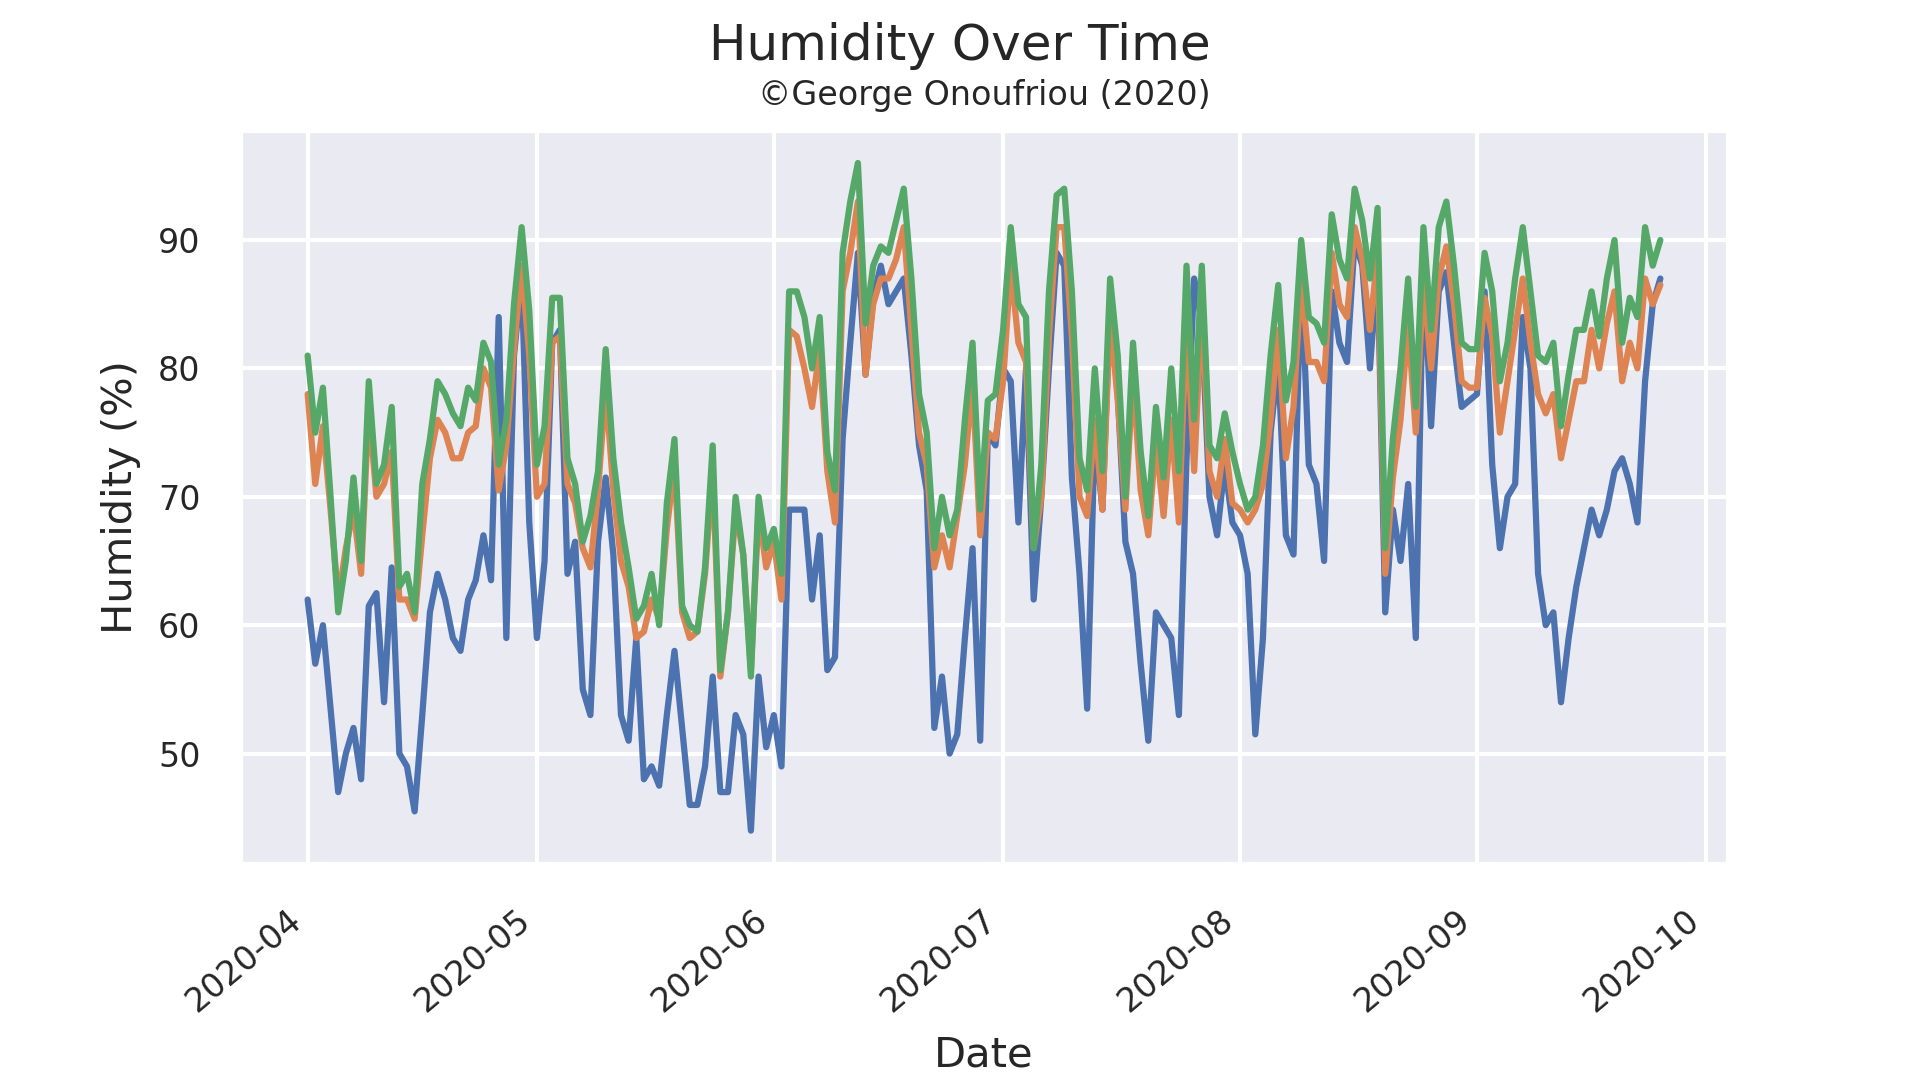
\includegraphics[origin=c,width=1\textwidth]{humidiy_over_time.png}
          \caption{Humidity over time in our riseholme campus (2020).}
          \label{fig:humidity}
        \end{figure}
      \end{column}
      \begin{column}{0.5\textwidth}
        \begin{figure}[th!]
          \centering
          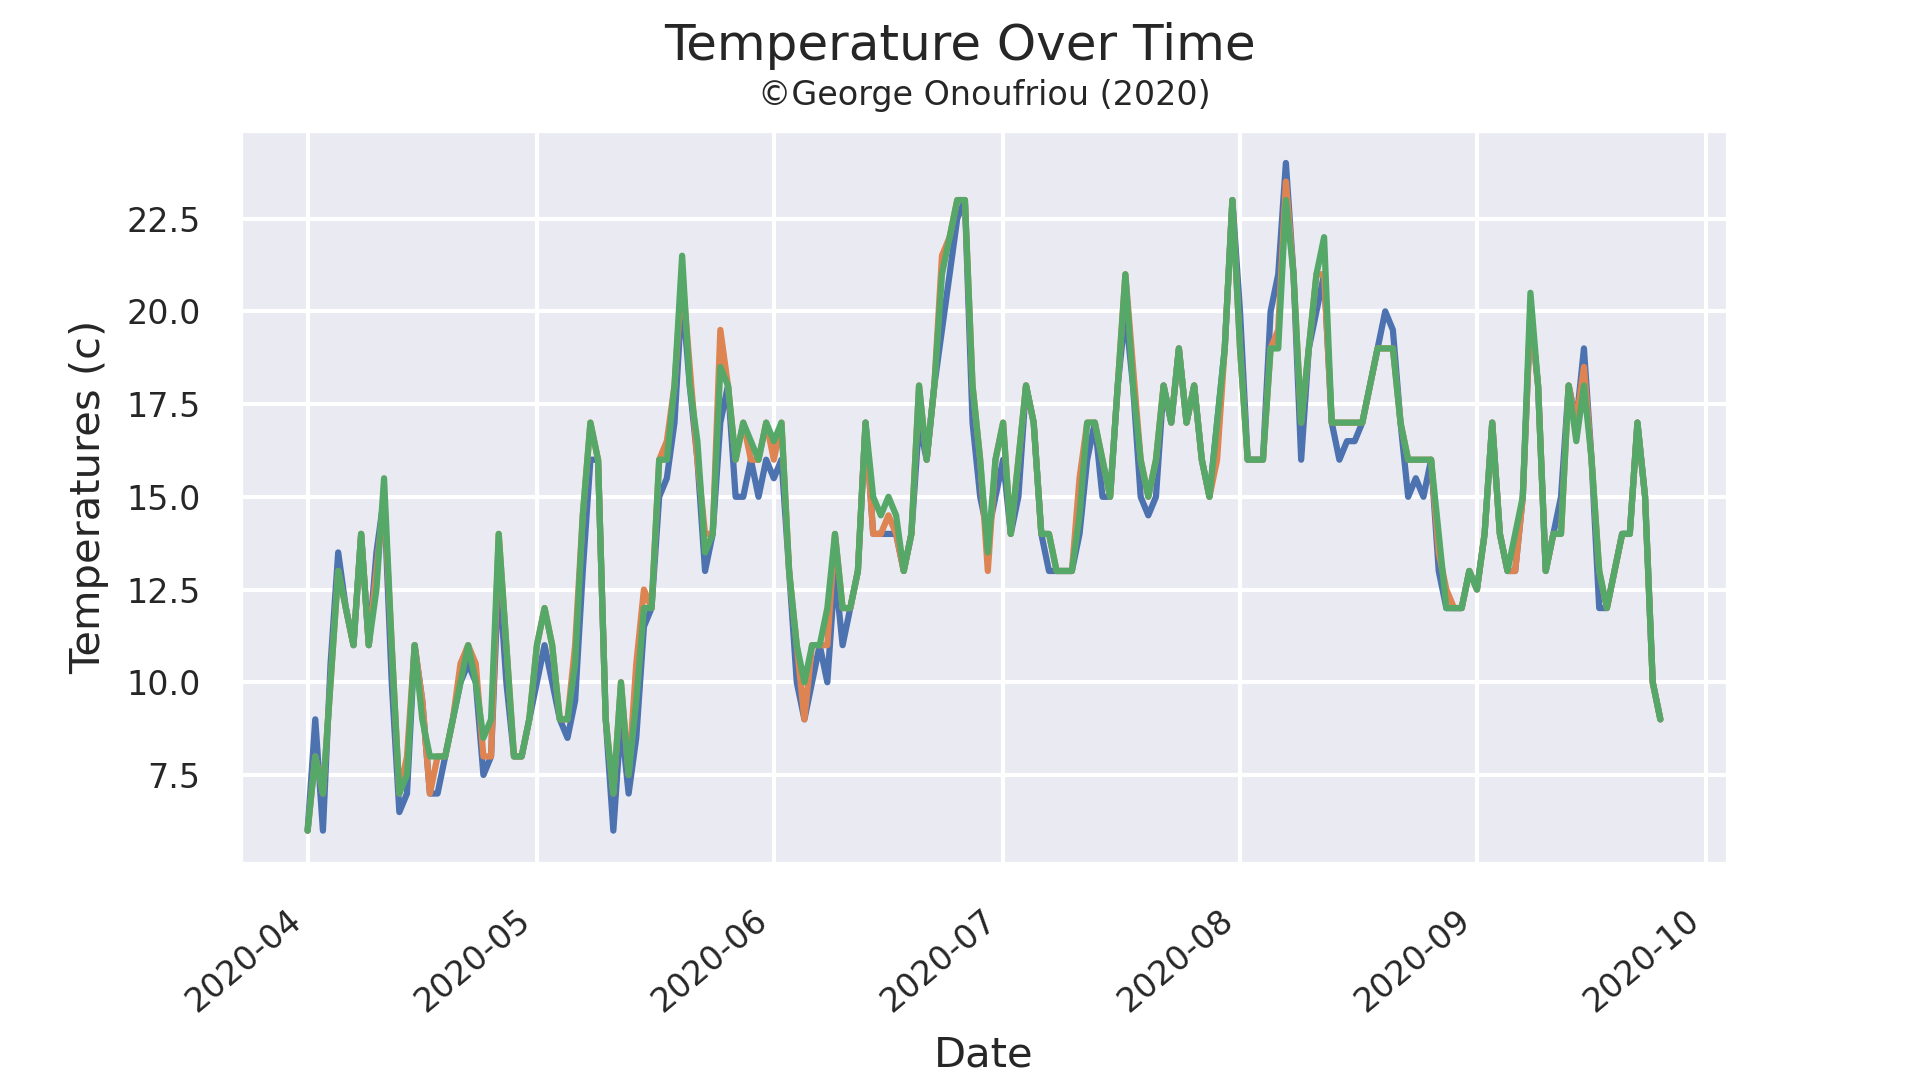
\includegraphics[origin=c,width=1\textwidth]{temp_over_time.png}
          \caption{Temperature over time in our riseholme campus (2020).}
          \label{fig:temp}
        \end{figure}
      \end{column}
    \end{columns}
  \end{frame}

  \begin{frame}
    Last years data collection, two weeks ahead:
    \begin{table}[]
      \begin{tabular}{l|l}
      Neural Network Type                   & Mean Absolute Error (MAE) Test Set \\ \hline
      Recurrent Neural Network (RNN)        & 0.208                              \\
      Long Short-Term Memory Network (LSTM) & 0.293                              \\
      Gated Recurrent Unit (GRU)            & 0.142
      \end{tabular}
    \end{table}
  \end{frame}

  % \begin{frame}[allowframebreaks]
  %   \frametitle{References}
  %   % % biblatex version
  %   \printbibliography
  % \end{frame}


\end{document}
